\section{Theorie}
\label{sec:Theorie}

Die vom $\gamma$- und $\beta$-Strahler der emittierten Photonen und Elektronen
wechselwirken mit Materie ausschließlich bei Stößen mit Teilchen.
Der Wirkungsquerschnitt $\delta$ stellt dabei ein Maß für die Häufigkeit von Wechselwirkungen dar.
Für einen Absorber der Dicke $D$ und eine infinitesimal dünne Schicht $\dif{x}$ des Absorbers gilt
\begin{equation}
    \dif{N} = -N(x) \, n \, \sigma \, \dif{x} \, .
\end{equation}
$N(x)$ beschreibt dabei die Strahlungsintensität und $\dif{N}$ die Abnahme der Teilchenzahl,
die hinter der Schicht $\dif{x}$ Impulse auslösen.
Durch Integration über alle Schichten $x \in [0, D]$ folgt das \textit{Absorptionsgesetz}
\begin{equation} \label{eq:absorptionsgesetz}
    N(D) = N_\text{0} \, e^{-n \sigma D} \, .
\end{equation}
Der Absorptionskoeffizient wird dabei durch $\mu = n \sigma$ beschrieben und 
$N_\text{0}$ ist die Zahl der ursprünglich vorhandenen Teilchen.
Das Absorptionsgesetz ist gültig, wenn jedes Teilchen nach einer Wechselwirkung
vernichtet wird oder die mittlere Entfernung zwischen zwei Reaktionen groß gegen $D$ ist.
Für $n$ gilt die Beziehung
\begin{equation} \label{eq:anzahl}
    n = \frac{z N_\text{A}}{V_\text{Mol}} = \frac{z N_\text{L} \rho}{M} \\
\end{equation}
mit den Zahlenwerten
\begin{align*}
    z                &\quad \text{Ordnungszahl}         \\
    N_\text{A}       &\quad \text{Avogadro-Konstante}   \\
    V_\text{Mol}     &\quad \text{Molvolumen}           \\
    M                &\quad \text{Molekulargewicht}     \\
    \rho             &\quad \text{Dichte des Absorbers} 
\end{align*}

\subsection[Gamma-Strahlung]{$\gamma$-Strahlung}

Bei dem Übergang eines Atomkerns von einem höheren Energieniveau zu einem niedrigeren
wird die frei werdende Energie in Form eines $\gamma$-Quants abgegeben. 
Diese Strahlung besteht aus Photonen und verhält sich entsprechend wie eine elektromagnetische Welle 
und die Energie eines Quants ist durch $E = h \mu$ gegeben. 
Das $\gamma$-Spektrum eines Kerns weist sehr scharfe Linien auf,
welche durch die präzise definierten Energieniveaus der Kerne zu erklären sind.

Für Energien zwischen $\qty{10}{keV}$ und $\qty{10}{MeV}$ treten abhängig vom Wechselwirkungs-Partner
verschiedene Effekte auf, welche in \autoref{fig:wwtabelle} zu sehen sind.
\begin{figure}
    \centering
    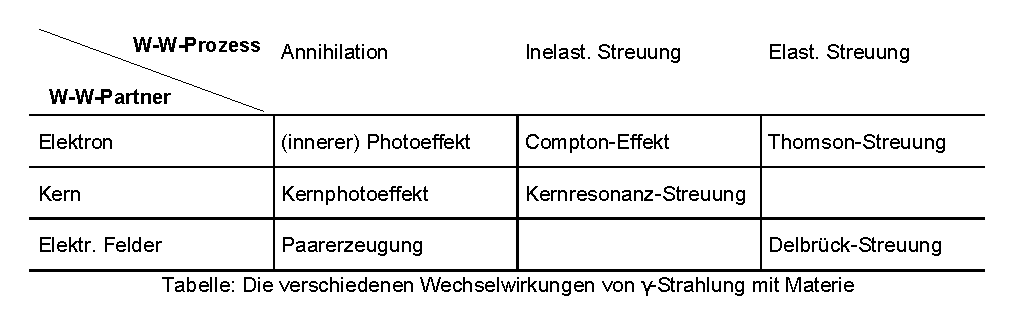
\includegraphics[width=\linewidth]{pictures/wwtabelle.pdf}
    \caption{Effekte durch Wechselwirkungen von $\gamma$-Quanten. \cite{v704}}
    \label{fig:wwtabelle}
\end{figure}